\documentclass[a4paper,14pt,russian]{article}
\usepackage{../MyPackages/commands}
\RequirePackage{caption}
\usepackage{graphicx}
\newcommand{\Pn}[3]{P^{(#1)} \br{#2,#3}}
\newcommand{\G}{\Gamma}
\newcommand{\e}{\eta_i^{(1)}}
\newcommand{\ee}{\eta_i^{(2)}}
\renewcommand{\b}{b^{(1)}}
\newcommand{\bb}{b^{(2)}}
\renewcommand{\P}[2]{P\br{\left. #1 \right| #2}}
\newcommand{\iakt}{[\tau_{i},\tau_{i+1})}
\newcommand{\Gr}[1]{\Gamma^{(#1)}}
\newcommand{\Mark}[0]{\brrr{\br{\G_i, \vk_{1,i}, \vk_{2,i}, \vk_{3,i}, \vk_{4,i}}, i \geqslant 0}}
%\newcommand{\Markk}[0]{\brrr{ \vk_i, i \geqslant 0}}
%\newcommand{\Markkhat}[0]{\brrr{ \hat{\vk}_i, i \geqslant 1}}
%\newcommand{\Markkhata}[0]{\brrr{ \hat{\vk}_i\br{a}, i \geqslant 1}}
%\newcommand{\Markkhato}[0]{\brrr{ \hat{\vk}_i\br{0}, i \geqslant 1}}
%\newcommand{\Markkhatoa}[0]{\brrr{ \hat{\hat{\vk}}_i\br{a}, i \geqslant 1}}
\usepackage[Magistr]{../MyPackages/ptvstyle}
%\selectlanguage{russian}
\title{Моделирование и анализ системы обслуживания конфликтных потоков в классе приоритетных алгоритмов}
\author{студент группы 85М1\\ Кочеганов В.~М.}
\advisor{к.ф.-м.н., доцент \\ Зорин А.~В.}
\chief{д.ф.-м.н., профессор \\ Федоткин М.~А.}
\date{2013}
\newcommand{\p}{\hat{p}}
\newcommand{\gam}[2]{\Gamma^{\left( #1 , #2 \right)} }
\newcommand{\T}[2]{T^{\left( #1 , #2 \right)} }
\newcommand{\ga}[1]{\Gamma^{\left( #1 \right)} }
\newcommand{\Tt}[1]{T^{\left( #1 \right)} }
\begin{document}

\section{Постановка задачи и построение математической модели}

\subsection{Постановка задачи на содержательном уровне}
Рассмотрим систему массового обслуживания следующего вида (Рис.~\ref{SystemScheme}).


\begin{figure}[h]
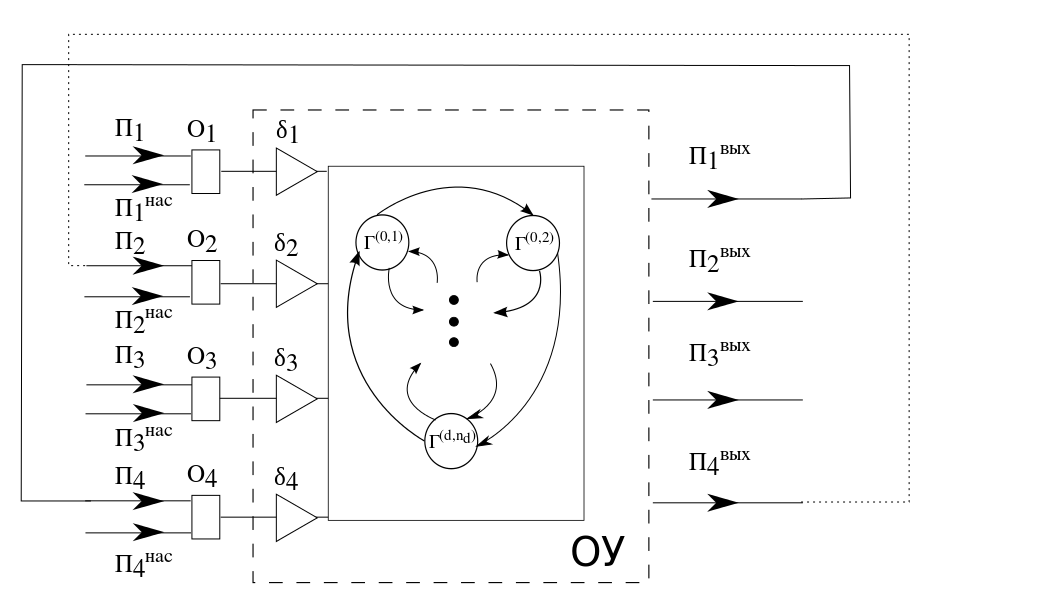
\includegraphics[scale=0.5]{SystemScheme.png} 
\caption{Структурная схема системы обслуживания}
\label{SystemScheme}
\end{figure}

Пусть в систему с одним обслуживающим устройством поступают потоки $\Pi_1$, $\Pi_2$, $\Pi_3$  и $\Pi_4$. Требования по потоку $\Pi_j$ становятся в соответствующую очередь $O_j$ неограниченной вместимостью, $j\in \brrr{1, 2, 3, 4}$. Для $j \in \brrr{1, 2, 3}$ дисциплина очереди $O_j$, поддерживаемая устройством $\delta_j$, имеет тип FIFO (First In First Out). Таким образом, для обслуживания из соответствующей очереди выбирается то требование, которое пришло раньше. Дисциплина очереди $O_4$ будет описана ниже. Входные потоки $\Pi_1$ и $\Pi_2$ формируются внешней средой, которая, будем предполагать, имеет только одно состояние, то есть вероятностная структура потоков не меняется с течением времени. Требования потоков $\Pi_1$ и $\Pi_3$ формируют независимые между собой неординарные пуассоновские потоки, то есть  стационарные, без последействия и ординарные потоки групп требований. Интенсивности соответствующих простейших потоков для $\Pi_1$ и $\Pi_3$ будем обозначать $\la_1$ и $\la_3$, а распределение числа заявок в группе по потоку $\Pi_j$ будем описывать производящей функцией
\begin{equation}
f_j(z) = \sum_{\nu=1}^{\infty} p_{\nu}^{(j)} z ^{\nu}
\end{equation}
 для $|z|<(1+\varepsilon), \varepsilon > 0$ и $p_{\nu}^{(j)}>0$. Величина $p_{\nu}^{(j)}$ определяет вероятность того, что по потоку $\Pi_j$ число требований в группе равно $\nu$, $j\in \brrr{1,3}$. Обслуженные требования потока $\Pi_1$ поступают на повторное обслуживание, формируя при этом поток $\Pi_4$ (т.е. $\Pi_1^{\mathrm{\text{вых}}} =  \Pi_4$). Далее, каждое требование из очереди $O_4$ с вероятностью $p_r$ и независимо от других завершает обслуживание и отправляется в очередь $O_2$ потока $\Pi_2$, где $r$~ --- номер состояния обслуживающего устройства на соответствующем такте обслуживания ($\Pi_4^{\mathrm{\text{вых}}}=\Pi_2$). С вероятностью $1-p_r$ требование очереди $O_4$ остается в ней до следующего такта. Потоки $\Pi_2$ и $\Pi_3$ являются конфликтными, что означает запрет на одновременное обслуживание требований этих потоков и, следовательно, исследование системы не может быть сведено к задаче с меньшим числом потоков. 
 
 В каждый момент времени обслуживающее устройство находится в одном из конечного множества состояний $\Gamma=\brrr{\Gr{1}, \Gr{2}, \ldots, \Gr{n}}$. В каждом состоянии $\ga{r}$ обслуживающее устройство находится в течение времени $\Tt{r}$. Множество $\G$ представим в виде суммы четырех непересекающихся подмножеств: $\G = \G^{\mathrm{\Rmnum{1}}} + \G^{\mathrm{\Rmnum{2}}} + \G^{\mathrm{\Rmnum{3}}} + \G^{\mathrm{\Rmnum{4}}}$, --- которые определим ниже.

В состоянии $\G^{(r)} \in \G^{\mathrm{\Rmnum{1}}}$ обслуживаются только требования из очередей $O_1$, $O_2$ и $O_4$.

В состоянии $\G^{(r)} \in \G^{\mathrm{\Rmnum{2}}}$ обслуживаются только требования из очередей $O_2$ и $O_4$.

В состоянии $\G^{(r)} \in \G^{\mathrm{\Rmnum{3}}}$ обслуживаются только требования из очередей $O_1$, $O_3$ и $O_4$.

В состоянии $\G^{(r)} \in \G^{\mathrm{\Rmnum{4}}}$ обслуживаются только требования из очередей $O_3$ и $O_4$.

Поскольку законы распределения выходных потоков, как правило, имеют сложный вид и часто не поддаются аналитическому выражению, вместо них будем использовать потоки насыщения $\Pi^{\mathrm{\text{нас}}}_j$, $j \in \brrr{1,2,3,4}$. Потоки насыщения $\Pi^{\mathrm{\text{нас}}}_j$, $j \in \brrr{1,2,3,4}$, представляют собой виртуальные выходные потоки при условии максимального использования ресурсов обслуживающего устройства, а для $j\in \brrr{1, 2, 3}$ еще и при условии максимальной загрузки соответствующих очередей. Пусть
\begin{equation}
^1\G=\G^{\mathrm{\Rmnum{1}}} \bigcup \G^{\mathrm{\Rmnum{3}}}, \quad
^2\G=\G^{\mathrm{\Rmnum{1}}} \bigcup \G^{\mathrm{\Rmnum{2}}}, \quad
^3\G=\G^{\mathrm{\Rmnum{3}}} \bigcup \G^{\mathrm{\Rmnum{4}}}.
\end{equation}
Тогда поток насыщения $\Pi^{\mathrm{\text{нас}}}_j$, $j\in \brrr{1,2,3}$, будет содержать неслучайное число $\ell_{r,j}$ требований, обслуженных в течение времени $\Tt{r}$, если $\ga{r} \in~ ^j\G$, и будет содержать $0$ требований в противном случае: $\ga{r} \notin ~ ^j\G$, $j\in \brrr{1,2,3}$. При условии, что в очереди $O_4$ находится $x \in Z_+$ требований, поток насыщения $\Pi^{\mathrm{\text{нас}}}_4$ определим как поток, содержащий все $x$ требований.

Для исследования системы обслуживания в данной работе будет использоваться так называемый кибернетический подход. В соответствии с этим подходом наблюдение за системой осуществляется в дискретные моменты времени $\tau_0 = 0,~ \tau_1,~ \ldots$,~  совпадающие с моментами переключения состояния обслуживающего устройства. 
Будем считать, что функция перехода из состояния $\G_i$ в момент $\tau_i$ в состояние $\G_{i+1}$ в момент $\tau_{i+1}$ известна и задается функцией $\G_{i+1} = h(\G_i,x_i)$ от предыдущего состояния $\G_i$ и величины $x_i$ очереди $O_3$ в момент $\tau_i$. Таким образом, обслуживающее устройство, в зависимости от объема очереди $O_3$, может переходить в разные состояния. Общая структура рассматриваемых графов переходов между состояниями будет описана ниже.

\subsection{Свойства условных распределений}

Все рассматриваемые в этой работе случайные элементы определяются на общем вероятностном пространстве $\br{\Omega, {\cal F}, P}$ элементарных исходов $\omega \in \Omega$ с вероятностной мерой $P(A)$, $A \in {\cal F}$ на $\sigma$-алгебре ${\cal F}$. Положим моменты наблюдения за системой 

Введем следующие случайные величины и элементы, $j \in \brrr{1,2,3,4}$:
\begin{itemize}
\item количество $\vk_{j,i} \in Z_+ $ требований в очереди $O_j$ в момент времени $\tau_i$;
\item состояние обслуживающего устройства $\G_i\in \G = \brrr{\G^{(1)},\G^{(2)}, \ldots, \G^{(n)}}$ в течение $\left(\tau_{i-1};\tau_i\right]$;
\item количество $\eta_{j,i}$ требований, поступивших в очередь $O_j$ по потоку $\Pi_j$ в течение $\left(\tau_{i};\tau_{i+1}\right]$;
\item количество $\xi_{j,i}$ требований по потоку насыщения $\Pi^{\mathrm{sat}}_j$ в течение $\left(\tau_{i};\tau_{i+1}\right]$;
\item количество $\overline{\xi}_{j,i}$ реально обслуженных требований по потоку $\Pi_j$.
\end{itemize}

Тогда для $j \in \brrr{1,2,3,4}$ имеем
\begin{equation}
\G_{i+1}=h(\G_i,\vk_{3,i}),\quad \vk_{j,i+1}=\max{\brrr{0,\vk_{j,i}+\eta_{j,i}-\xi_{j,i}}}, \quad \overline{\xi}_{j,i} = \min{\brrr{\xi_{j,i},\vk_{j,i}+\eta_{j,i}}}
\label{deterministicLawOne}
\end{equation}
и 
\begin{equation}
\eta_{2,i} = \overline{\xi}_{4,i}, \quad \eta_{4,i}=\overline{\xi}_{1,i}.
 \label{deterministicLawTwo}
\end{equation}
Также для определения длительности $T_{i}$ состояния обслуживающего устройства в течение $\left(\tau_{i-1};\tau_i\right]$, удобно ввести функцию $h_T(\cdot,\cdot)$:
\begin{equation}
T_{i+1}=h_T(\G_i,\vk_{3,i})= \Tt{r'},\quad  \text{ где } \ga{r'}=h(\G_i,\vk_{3,i}).
\label{timeLaw}
\end{equation}

Обозначим через $\vp_j(x,t)$, $j\in \brrr{1,3}$, условную вероятность того, что за время $t>0$ по потоку $\Pi_j$ поступит ровно $b\in Z_+$ требований:
\begin{equation}
\P{\brrr{\omega\colon \eta_{j,i} = b}}{\brrr{\omega\colon \G_i=\ga{r}, \vk_{3,i}=x}}=\vp_j(b,h_T (\ga{r}, x)).
\end{equation}
Учитывая закон распределения процесса Пуассона и количества требований в пачках, величины $\vp_j(x,t)$ могут быть найдены из соотношений
\begin{equation}
\sum_{x=0}^{\infty} z^x\vp_j(x,t) = exp\brrr{\la_j t \br{\sum_{b=1}^{\infty} z^b \pi(b,j) -1}}.
\end{equation}

Для потоков насыщения имеем следующие соотношения:
\begin{align}
\P{\xi_{j,i} = 0}{\G_i=\ga{r}, \vk_{3,i} = x} = 1, &\quad \G_{i+1} \notin~^j\G,\\
\P{\xi_{j,i} = l_{r',j}}{\G_i=\ga{r}, \vk_{3,i} = x} = 1, &\quad \G_{i+1}=\ga{r'}\in~^j\G,
\end{align}
где $j\in \{1, 2, 3\}$, $x \in Z_+$.

Введем для $0 < u \leqslant 1$ и $0 \leqslant k \leqslant x$ величину
\begin{equation}
\psi\br{k,x,u} = C_x^k u^k (1-u)^{x-k}.
\end{equation}
Поскольку требования из очереди $O_4$ независимо друг от друга с вероятностью $p_r$ на выходе системы (т.е. в результате обслуживания) поступают в очередь $O_2$, то количество требований в выходном потоке $\Pi_4^{\mathrm{out}}$ определяется по биномиальному закону распределения:
\begin{equation}
\P{\overline{\xi}_{4,i} = b}{ \G_i = \ga{r}, \vk_{4,i}=x, \vk_{3,i}=\tilde{x}}=\psi\br{b,x,p_{r'}}, \quad \G_{i+1}=\ga{r'}, \quad 0 \leqslant b \leqslant x.
\end{equation}


Введем следующие события:
\begin{align}
A_i\br{r;x_1;x_2;x_3;x_4} &= \brrr{\G_i=\ga{r},\vk_{3,i}=x_3}\bigcap \brrr{\vk_{1,i}=x_1,\vk_{2,i}=x_2,\vk_{4,i}=x_4}\\
B_i\br{b_1;b_2;b_3;y_1;y_2;y_3} &= \brrr{\eta_{1,i}=b_1,\eta_{2,i}=b_2,\eta_{3,i}=b_3,\xi_{1,i}=y_1,\xi_{2,i}=y_2,\xi_{3,i}=y_3}
\end{align}

В соответствии с описанной структурой системы, количество требований пришедших по потокам $\Pi_1$, $\Pi_2$, $\Pi_3$, $\Pi_4$, $\Pi_1^{\mathrm{\text{нас}}}$, $\Pi_2^{\mathrm{\text{нас}}}$ и $\Pi_3^{\mathrm{\text{нас}}}$ за $(i+1)$-ый такт зависит лишь от состояния обслуживающего устройства и размера очереди $O_3$ в момент $\tau_i$. Поэтому условные распределения рассматриваемых в системе потоков, учитывая все <<прошлое>> системы можно расписать следующим образом:
\ml
{
\label{etaXiIndependence}
\P{B_i\br{b_1;b_2;b_3;y_1;y_2;y_3}}{\bigcap_{t=0}^{i} A_t\br{r_t;x_{1,t};x_{2,t};x_{3,t};x_{4,t}}} = \\
= \P{\eta_{1,i}=b_1, \eta_{2,i}=b_2,\eta_{3,i}=b_3, \xi_{1,i}=y_1, \xi_{2,i}=y_2, \xi_{3,i}=y_3}{\G_i=\ga{r_i},\vk_{3,i}=x_{3,i}}=\\
= \P{\eta_{1,i}=b_1}{\G_i=\ga{r_i},\vk_{3,i}=x_{3,i}} \times
\P{\eta_{2,i}=b_2}{\G_i=\ga{r_i},\vk_{3,i}=x_{3,i}} \times \\
\P{\eta_{3,i}=b_3}{\G_i=\ga{r_i},\vk_{3,i}=x_{3,i}} \times 
\P{\xi_{1,i}=y_1}{\G_i=\ga{r_i},\vk_{3,i}=x_{3,i}} \times \\
\P{\xi_{2,i}=y_2}{\G_i=\ga{r_i},\vk_{3,i}=x_{3,i}} \times 
\P{\xi_{3,i}=y_3}{\G_i=\ga{r_i},\vk_{3,i}=x_{3,i}}
}

Сформулируем и докажем теорему о марковости последовательности $\Mark$:
\begin{theorem}
При заданном распределении начального вектора $\br{\G_0,\vk_{1,0},\vk_{2,0},\vk_{3,0},\vk_{4,0}}$ последовательность $\Mark$ является цепью Маркова. 
\end{theorem}

\begin{proof}
Для доказательства достаточно показать, что 
\ml
{
\P{A_{i+1}\br{r;x_{1};x_{2};x_{3};x_{4}}}{\bigcap_{t=0}^{i} A_t\br{r_t;x_{1,t};x_{2,t};x_{3,t};x_{4,t}}} = \\
\P{A_{i+1}\br{r;x_{1};x_{2};x_{3};x_{4}}}{ A_i\br{r_i;x_{1,i};x_{2,i};x_{3,i};x_{4,i}}}
\label{markovToProve}
}
Распишем сначала левую часть равенства \eqref{markovToProve}. Учитывая то, что сумма непересекающихся событий $B_i\br{b_1;b_2;b_3;y_1;y_2;y_3}$ есть достоверное событие, $\bigcup_{b,y} B_i\br{b_1;b_2;b_3;y_1;y_2;y_3}=\Omega$ получим

\ml
{
\P{A_{i+1}\br{r;x_{1};x_{2};x_{3};x_{4}}}{\bigcap_{t=0}^{i} A_t\br{r_t;x_{1,t};x_{2,t};x_{3,t};x_{4,t}}} = \\
=\sum_{b,y}\P{A_{i+1}\br{r;x_{1};x_{2};x_{3};x_{4}} \bigcap B_i\br{b_1;b_2;b_3;y_1;y_2;y_3}}{\bigcap_{t=0}^{i} A_t\br{r_t;x_{1,t};x_{2,t};x_{3,t};x_{4,t}}} = \\
= \sum_{b,y}\P{B_i\br{b_1;b_2;b_3;y_1;y_2;y_3}}{\bigcap_{t=0}^{i} A_t\br{r_t;x_{1,t};x_{2,t};x_{3,t};x_{4,t}}}\times\\
\times \P{A_{i+1}\br{r;x_{1};x_{2};x_{3};x_{4}}}{\bigcap_{t=0}^{i} A_t\br{r_t;x_{1,t};x_{2,t};x_{3,t};x_{4,t}}\bigcap B_i\br{b_1;b_3;b_3;y_1;y_2;y_3}}
\label{markovProof}
}
Беря во внимание \eqref{deterministicLawOne} и \eqref{deterministicLawTwo}, найдем второй множитель:
\ml
{
\P{A_{i+1}\br{r;x_{1};x_{2};x_{3};x_{4}}}{\bigcap_{t=0}^{i} A_t\br{r_t;x_{1,t};x_{2,t};x_{3,t};x_{4,t}}\bigcap B_i\br{b_1;b_2;b_3;y_1;y_2;y_3}} = \\
= P\left(\G_{i+1}=\ga{r},\vk_{1,i+1}=x_1,\vk_{2,i+1}=x_2,\vk_{3,i+1}=x_3,\vk_{4,i+1}=x_4\right| \bigcap_{t=0}^{i-1} A_t\br{r_t;x_{1,t};x_{2,t};x_{3,t};x_{4,t}} \bigcap \\ \bigcap 
\brrr{\G_i=\ga{r_i},\vk_{1,i}=x_{1,i},\vk_{2,i}=x_{2,i},\vk_{3,i}=x_{3,i},\vk_{4,i}=x_{4,i}} \bigcap \\
\bigcap \left. \brrr{\eta_{1,i}=b_1,\eta_{2,i}=b_2,\eta_{3,i}=b_3,\xi_{1,i}=y_1,\xi_{2,i}=y_2,\xi_{3,i}=y_3}
\right) = \\
= P\left(h\br{\ga{r_i},x_{3,i}}=\ga{r},
\max{\brrr{0,x_{1,i}+b_1-y_1}}=x_1,\right.\\
\max{\brrr{0,x_{4,i}+\min{\brrr{y_1,x_{1,i}+b_1}} - y_3}}=x_4,
\max{\brrr{0,x_{2,i}+b_2-y_2}}=x_2, \\
\left.
\max{\brrr{0,x_{3,i}+b_3-y_2}}=x_3,\right| 
\bigcap_{t=0}^{i-1} A_t\br{r_t;x_{1,t};x_{2,t};x_{3,t};x_{4,t}} \bigcap\\
\bigcap 
\brrr{\G_i=\ga{r_i},\vk_{1,i}=x_{1,i},\vk_{2,i}=x_{2,i},\vk_{3,i}=x_{3,i},\vk_{4,i}=x_{4,i}} \bigcap \\
\bigcap \left. \brrr{\eta_{1,i}=b_1,\eta_{2,i}=b_2,\eta_{3,i}=b_3,\xi_{1,i}=y_1,\xi_{2,i}=y_2,\xi_{3,i}=y_3}
\right) = \\ 
= P\left(h\br{\ga{r_i},x_{3,i}}=\ga{r},
\max{\brrr{0,x_{1,i}+b_1-y_1}}=x_1,\right.\\
\max{\brrr{0,x_{4,i}+\min{\brrr{y_1,x_{1,i}+b_1}} - y_3}}=x_4,
\max{\brrr{0,x_{2,i}+b_2-y_2}}=x_2, \\
\left.
\max{\brrr{0,x_{3,i}+b_2-y_2}}=x_3\right),
\label{markovProoff}
}
где последнее равенство верно, поскольку оставшаяся под знаком вероятности величина уже не является случайной. Из \eqref{etaXiIndependence}, \eqref{markovProof} и  \eqref{markovProoff} получаем выражение для левой части равенства \eqref{markovToProve}:
\ml
{
\P{A_{i+1}\br{r;x_{1};x_{2};x_{3};x_{4}}}{\bigcap_{t=0}^{i} A_t\br{r_t;x_{1,t};x_{2,t};x_{3,t};x_{4,t}}} = \\
=  \sum_{b,y}\P{\eta_{1,i}=b_1, \eta_{2,i}=b_2, \eta_{3,i}=b_3, \xi_{1,i}=y_1, \xi_{2,i}=y_2, \xi_{3,i}=y_3}{\G_i=\ga{r_i},\vk_{3,i}=x_{3,i}}\times\\
\times  P\left(h\br{\ga{r_i},x_{3,i}}=\ga{r},
\max{\brrr{0,x_{1,i}+b_1-y_1}}=x_1,\right.\\
\max{\brrr{0,x_{4,i}+\min{\brrr{y_1,x_{1,i}+b_1}} - y_3}}=x_4,
\max{\brrr{0,x_{2,i}+b_2-y_2}}=x_2, \\
\left.
\max{\brrr{0,x_{3,i}+b_2-y_2}}=x_3\right)
}

Заметим, что в наших рассуждениях мы нигде не использовали информацию о событиях \par $\bigcap_{t=0}^{i-1} A_t\br{r_t;x_{1,t};x_{2,t};x_{3,t};x_{4,t}}$, поэтому рассуждения для правой части \eqref{markovToProve} будут аналогичными:
\mll
{
\P{A_{i+1}\br{r;x_{1};x_{2};x_{3};x_{4}}}{ A_i\br{r_i;x_{1,i};x_{2,i};x_{3,i};x_{4,i}}} = \\
= \sum_{b,y}\P{B_i\br{b_1;b_2;b_3;y_1;y_2;y_3}}{ A_i\br{r_i;x_{1,i};x_{2,i};x_{3,i};x_{4,i}}}\times\\
\times \P{A_{i+1}\br{r;x_{1};x_{2};x_{3};x_{4}}}{ A_i\br{r_i;x_{1,i};x_{2,i};x_{3,i};x_{4,i}}\bigcap B_i\br{b_1;b_2;b_3;y_1;y_2;y_3}} = \\
= \sum_{b,y}\P{\eta_{1,i}=b_1, \eta_{2,i}=b_2, \eta_{3,i}=b_3, \xi_{1,i}=y_1, \xi_{2,i}=y_2, \xi_{3,i}=y_3}{\G_i=\ga{r_i},\vk_{3,i}=x_{3,i}}\times \\
\times 
P\left(\G_{i+1}=\ga{r},\vk_{1,i+1}=x_1,\vk_{2,i+1}=x_2,\vk_{3,i+1}=x_3,\vk_{4,i+1}=x_4\right|  \\ 
\brrr{\G_i=\ga{r_i},\vk_{1,i}=x_{1,i},\vk_{2,i}=x_{2,i},\vk_{3,i}=x_{3,i},\vk_{4,i}=x_{4,i}} \bigcap \\
\bigcap \left. \brrr{\eta_{1,i}=b_1,\eta_{2,i}=b_2,\eta_{3,i}=b_3,\xi_{1,i}=y_1,\xi_{2,i}=y_2,\xi_{2,i}=y_2,\xi_{3,i}=y_3}
\right) = 
}
откуда опять в силу \eqref{deterministicLawOne} и \eqref{deterministicLawTwo} получаем
\mll
{
=\sum_{b,y}\P{\eta_{1,i}=b_1, \eta_{2,i}=b_2, \eta_{3,i}=b_3, \xi_{1,i}=y_1, \xi_{2,i}=y_2, \xi_{3,i}=y_3}{\G_i=\ga{r_i},\vk_{3,i}=x_{3,i}}\times \\
\times P\left(h\br{\ga{r_i},x_{3,i}}=\ga{r},
\max{\brrr{0,x_{1,i}+b_1-y_1}}=x_1,\right.\\
\max{\brrr{0,x_{4,i}+\min{\brrr{y_1,x_{1,i}+b_1}} - y_3}}=x_4,
\max{\brrr{0,x_{2,i}+b_2-y_2}}=x_2, \\
\left.
\max{\brrr{0,x_{3,i}+b_2-y_2}}=x_3\right).
}
Таким образом, выражения для левой и правой частей \eqref{markovToProve} совпадают, следовательно равенство верно и последовательность $\Mark$ является цепью Маркова.
\end{proof}


\end{document}






\subsection{Постановка задачи}

\begin{figure}[h]
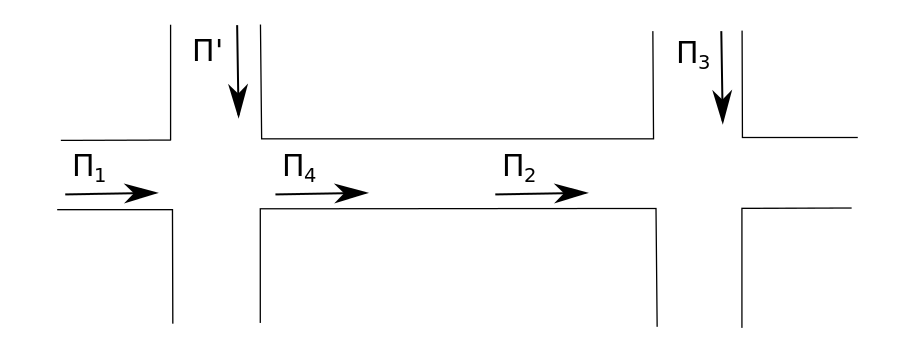
\includegraphics[scale=0.5]{Crossroads.png} 
\end{figure}

\begin{figure}[h]
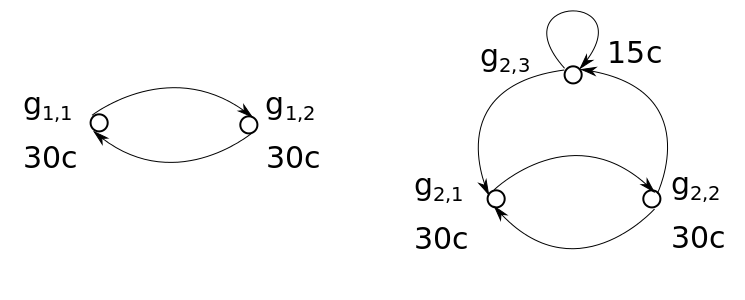
\includegraphics[scale=0.5]{SystemStates.png} 
\end{figure}



Требования по потокам $\Pi_j$, $j=1,2,4$, поступают пачками, причем пачки поступают в соответствии с Пуассоновским процессом с параметром $\la_j$. Требования из потока $\Pi_1$, будучи обслуженными, образуют поток $\Pi_3$.
Требования по потоку $\Pi_j$ поступают в соответствующую очередь $O_j$, $j=\overline{1,4}$.

Первый перекресток может находиться в одном из двух состояний:
\begin{itemize}
\item обслуживать поток $\Pi_1$ (состояние $\gam{1}{1}$ длительностью $\T{1}{1}$) и 
\item
обслуживать поток $\Pi_2$ (состояние $\gam{1}{2}$ длительностью $\T{1}{2}$).
\end{itemize}

Второй перекресток имеет три состояния:
\begin{itemize}
\item обслуживание потока $\Pi_3$ (состояние $\gam{2}{1}$ длительностью $\T{2}{1}$);
\item обслуживание потока $\Pi_4$ (состояние $\gam{2}{2}$ длительностью $\T{2}{2}$) и
\item продолжение обслуживания потока $\Pi_4$ в случае 
превышения объема оставшейся очереди $O_4$ некого порога (состояние $\gam{2}{3}$ длительностью $\T{2}{3}$);
\end{itemize}

Объединим рассматриваемые обслуживающие устройства в одно, состояние которого опишем с помощью вектора из множества $S_{general}\left(\Gamma^{(1,i_1)}; \Gamma^{(2,i_2)}; T\right)$, где $i_1\in \left\{1,2\right\}$, $i_2 \in \left\{1,2,3\right\}$, $T\in \left\{1, 2, \ldots, \max_{i_1,i_2}{\left(T^{(1,i_1)}, T^{(2,i2)}\right)}\right\}$. Свое состояние новое устройство меняет в моменты смены состояний одного из составляющих его устройств.

\begin{theorem}
Количество состояний полученного обслуживающего устройства конечно
\end{theorem}
\begin{proof}
Поскольку множество различных состояний $\Gamma$, в которые обслуживающее устройство может совершить переход, является подмножеством $S_{general}$ ($S \subset S_{general}$), то
\begin{equation*}
\left|S\right| \leqslant \left|S_{general}\right| = 2\times 3 \times \max_{i_1,i_2}{\left(T^{(1,i_1)}, T^{(2,i2)}\right)}
\end{equation*}
\end{proof}

В следствие этого результата мы можем перенумеровать состояния $\G = \brrr{\G^{(1)},\G^{(2)}, \ldots, \G^{(n)}}$, а также соответствующие им длительности $T=\brrr{T^{(1)},T^{(2)}, \ldots, T^{(n)}}$.
Каждое состояние $\G^{(r)}$ принадлежит одному из следующих четырех классов $\G^{\mathrm{\Rmnum{1}}}$, $\G^{\mathrm{\Rmnum{2}}}$, $\G^{\mathrm{\Rmnum{3}}}$ и $\G^{\mathrm{\Rmnum{4}}}$.
\begin{itemize}
\item в состоянии $\G^{(r)} \in \G^{\Rmnum{1}}$ обслуживаются только требования из очередей $O_1$ и $O_3$;
\item в состоянии $\G^{(r)} \in \G^{\Rmnum{2}}$ обслуживаются только требования из очередей $O_1$ и $O_4$;
\item в состоянии $\G^{(r)} \in \G^{\Rmnum{3}}$ обслуживаются только требования из очередей $O_2$ и $O_3$;
\item в состоянии $\G^{(r)} \in \G^{\Rmnum{4}}$ обслуживаются только требования из очередей $O_2$ и $O_4$.
\end{itemize}

Для описания процесса обслуживания будут также использоваться потоки насыщения $\Pi^{\mathrm{sat}}_j$, $j=\overline{1,4}$, определяемые как выходные потоки при максимальной загруженности обслуживающего устройства. Пусть
\begin{itemize}
\item для $j=1$ $^j\G=\G^{\Rmnum{1}} \bigcup \G^{\Rmnum{2}}$;
\item для $j=2$ $^j\G=\G^{\Rmnum{3}} \bigcup \G^{\Rmnum{4}}$;
\item для $j=3$ $^j\G=\G^{\Rmnum{1}} \bigcup \G^{\Rmnum{3}}$;
\item для $j=4$ $^j\G=\G^{\Rmnum{2}} \bigcup \G^{\Rmnum{4}}$;
\end{itemize}
Тогда поток насыщения $\Pi^{\mathrm{sat}}_j$ будет содержать неслучайное число $l_{r,j}$ требований, обслуженных в течение времени $\Tt{r}$, если $\ga{r} \in ^j\G$, и не будет содержать требований в противном случае, $\ga{r} \notin ^j\G$. 

Моменты $\tau_0 = 0, \tau_1, \ldots$ наблюдения за системой положим совпадающими с моментами переключения состояния обслуживающего устройства. Определим следующие случайные величины и элементы:
\begin{itemize}
\item количество $\vk_{j,i} \in Z_+ $ требований в очереди $O_j$ в момент времени $\tau_i$;
\item состояние обслуживающего устройства $\G_i\in \G = \brrr{\G^{(1)},\G^{(2)}, \ldots, \G^{(n)}}$ в течение $\left(\tau_{i-1};\tau_i\right]$;
\item количество $\eta_{j,i}$ требований, поступивших в очередь $O_j$ по потоку $\Pi_j$ в течение $\left(\tau_{i};\tau_{i+1}\right]$;
\item количество $\xi_{j,i}$ требований по потоку насыщения $\Pi^{\mathrm{sat}}_j$ в течение $\left(\tau_{i};\tau_{i+1}\right]$;
\item количество $\overline{\xi_{j,i}}$ реально обслуженных требований по потоку $\Pi_j$,
\end{itemize}
для $j=\overline{1,4}$.





